\section{Tau-Tau Plots}
    \begin{frame}[plain]
        \vfill
      \centering
      \begin{beamercolorbox}[sep=8pt,center,shadow=true,rounded=true]{title}
        \usebeamerfont{title}\insertsectionhead\par%
        \color{oxfordblue}\noindent\rule{10cm}{1pt} \\
        \begin{itemize}
        \item As we already noted $\tau$ goes approximately quadratically with $U$.
        \item Decomposed into $\tau_u$, $\tau_v$ (along u, v axes).
        \item Regressing $\Delta\eta_{\quad hp}$ against $\tau_u$ and $\tau_v$ seems to
         reveal a linear relationship, most clear at vulnerable sights (New Orleans).
        \item How much of a difference does Robust vs. Standard Linear Regression make?
        \end{itemize}
       % 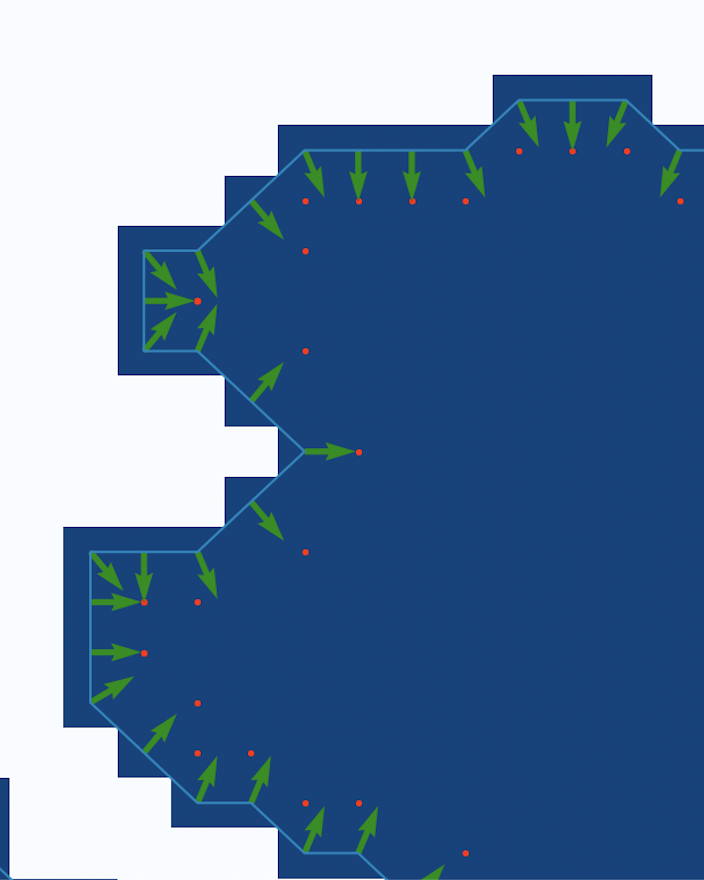
\includegraphics[width=0.4\linewidth]{images/example-images/new-orleans-example.png}
        %\includegraphics[width=0.52\linewidth]{../surge/plots/angles_hist.pdf}
      \end{beamercolorbox}
      \vfill
  \end{frame}

\begin{frame}{New Orleans $\Delta\eta$ or $\Delta\eta_{\;\;\mathrm{hp}}$ against $\tau_u$, or $\tau_v$}
\vspace{-30pt}
    %\centering
\hspace{-30pt}
 \begin{minipage}{1.15\textwidth}
\begin{figure}[htb!]
    \centering
   \hspace{-40pt} \includegraphics[width=0.42\linewidth]{../surge/plots/tau-tau/norlean-u.pdf}
        \includegraphics[width=0.42\linewidth]{../surge/plots/tau-tau/norlean-v.pdf}

   \hspace{-40pt} \includegraphics[width=0.42\linewidth]{../surge/plots/tau-tau-hp/norlean-u.pdf}
        \includegraphics[width=0.42\linewidth]{../surge/plots/tau-tau-hp/norlean-v.pdf}
    \vspace{-15pt}
    \caption{High pass filter changes New Orleans little.}
    \label{fig:A}
\end{figure}
\end{minipage}
\end{frame}

\begin{frame}{Miami $\Delta\eta$ or $\Delta\eta_{\;\;\mathrm{hp}}$ against $\tau_u$, or $\tau_v$}
\vspace{-30pt}
    %\centering
\hspace{-30pt}
 \begin{minipage}{1.1\textwidth}
\begin{figure}[htb!]
    \centering
   \hspace{-40pt} \includegraphics[width=0.42\linewidth]{../surge/plots/tau-tau/miami-u.pdf}
        \includegraphics[width=0.42\linewidth]{../surge/plots/tau-tau/miami-v.pdf}

   \hspace{-40pt} \includegraphics[width=0.42\linewidth]{../surge/plots/tau-tau-hp/miami-u.pdf}
        \includegraphics[width=0.42\linewidth]{../surge/plots/tau-tau-hp/miami-v.pdf}
    \vspace{-15pt}
    \caption{High pass filter makes Miami more New Orleans like.}
    \label{fig:A}
\end{figure}
\end{minipage}
\end{frame}


\begin{frame}{New York $\Delta\eta$ or
              $\Delta\eta_{\;\;\mathrm{hp}}$ against $\tau_u$, or $\tau_v$}
\vspace{-30pt}
    %\centering
\hspace{-30pt}
 \begin{minipage}{1.1\textwidth}
\begin{figure}[htb!]
    \centering
   \hspace{-40pt} \includegraphics[width=0.42\linewidth]{../surge/plots/tau-tau/new-york-u.pdf}
        \includegraphics[width=0.42\linewidth]{../surge/plots/tau-tau/new-york-v.pdf}

   \hspace{-40pt} \includegraphics[width=0.42\linewidth]{../surge/plots/tau-tau-hp/new-york-u.pdf}
        \includegraphics[width=0.42\linewidth]{../surge/plots/tau-tau-hp/new-york-v.pdf}
    \vspace{-15pt}
    \caption{High pass filter (lower two panels) makes small difference.}
    \label{fig:A}
\end{figure}
\end{minipage}
\end{frame}

\section{But these plots all had high excess kurtosis on all variables!  }
    \begin{frame}[plain]
        \vfill
      \centering
      \begin{beamercolorbox}[sep=8pt,center,shadow=true,rounded=true]{title}
        \usebeamerfont{title}\insertsectionhead\par%
        \color{oxfordblue}\noindent\rule{10cm}{1pt} \\
        \begin{itemize}
        \item$\mathbb{P}(\mathrm{Gaussian})<10^{-304}$ etc.
        \item The variables are also not necessarily positive (so no $\log$ trick).
        \item It would be interesting to see if there is a warping function
         that can do this (Extreme Value Textbooks are being rapidly skimmed).
        \item E.g .       \begin{equation}
       x^{\prime} = \tanh{\frac{x}{2\sigma_x}} \text{}
       \end{equation}
       Does make the distributions more normal.
        \end{itemize}
       % 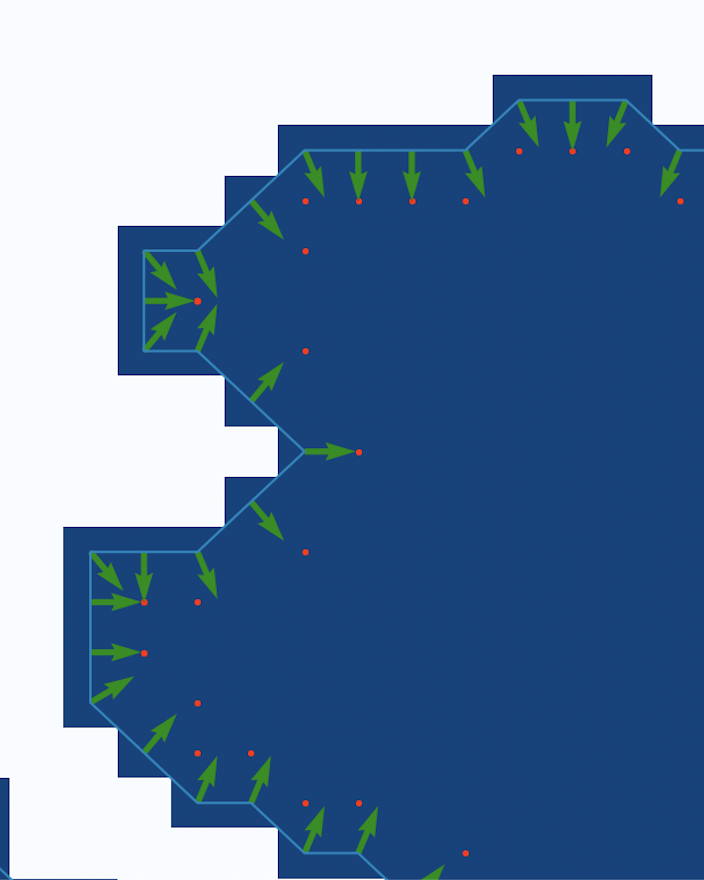
\includegraphics[width=0.4\linewidth]{images/example-images/new-orleans-example.png}
        %\includegraphics[width=0.52\linewidth]{../surge/plots/angles_hist.pdf}
      \end{beamercolorbox}
      \vfill
  \end{frame}


\begin{frame}{New York $\Delta\eta_{\;\;\mathrm{hp}}$ against $\tau_u$, and $\tau_v$}
\vspace{-30pt}
    %\centering
\hspace{-30pt}
 \begin{minipage}{1.1\textwidth}

\begin{figure}[htb!]
    \centering
   \hspace{-40pt} \includegraphics[width=1\linewidth]{../surge/plots/3d_plots/3d_plotnew-york.pdf}
    \vspace{-15pt}
   % \caption{High pass filter (lower two panels) makes small difference.}
    \label{fig:A}
\end{figure}
\end{minipage}
\end{frame}


\begin{frame}{Miami $\Delta\eta_{\;\;\mathrm{hp}}$ against $\tau_u$, and $\tau_v$}
\vspace{-30pt}
    %\centering
\hspace{-30pt}
 \begin{minipage}{1.1\textwidth}

\begin{figure}[htb!]
    \centering
   \hspace{-40pt} \includegraphics[width=1\linewidth]{../surge/plots/3d_plots/3d_plotmiami.pdf}
    \vspace{-15pt}
    \caption{Most variance not attributable to wind stress.}
    \label{fig:A}
\end{figure}
\end{minipage}
\end{frame}


\begin{frame}{New Orleans $\Delta\eta_{\;\;\mathrm{hp}}$ against $\tau_u$, and $\tau_v$}
\vspace{-30pt}
    %\centering
\hspace{-30pt}
 \begin{minipage}{1.1\textwidth}
\begin{figure}[htb!]
    \centering
   \hspace{-40pt} \includegraphics[width=1\linewidth]{../surge/plots/3d_plots/3d_plotnorlean.pdf}
    \vspace{-15pt}
   % \caption{High pass filter (lower two panels) makes small difference.}
    \label{fig:A}
\end{figure}
\end{minipage}
\end{frame}


\begin{frame}{Regression Summarised for Every Point.}
\vspace{-30pt}
    %\centering
\hspace{-30pt}
 \begin{minipage}{1.1\textwidth}
\begin{figure}[htb!]
    \centering
   \hspace{-40pt} \includegraphics[width=0.7\linewidth]{../surge/plots/rmlr.pdf}
    \vspace{-15pt}
   \caption{Huber regression generalises less well than MLR.}
    \label{fig:A}
\end{figure}
\end{minipage}
\end{frame}


\section{So it seems that in vulnerable places,
         a  majority of the variance can be predicted by $\tau_u$, and $\tau_v$.}
    \begin{frame}[plain]
        \vfill
      \centering
      \begin{beamercolorbox}[sep=8pt,center,shadow=true,rounded=true]{title}
        \usebeamerfont{title}\insertsectionhead\par%
        \color{oxfordblue}\noindent\rule{10cm}{1pt} \\
        \begin{itemize}
        \item Huber regression (supposedly more robust) does not significantly change the results.
        \item Approximately the same linear model is learnt, independent of year trained on.
        \item Miami, and the point near New Orleans stick out as places of poor fit.
        \end{itemize}
      \end{beamercolorbox}
      \vfill
  \end{frame}


  \begin{frame}{Orientation of the Regression Line}
\vspace{-30pt}
\hspace{-30pt}
 \begin{minipage}{1.1\textwidth}
 \begin{minipage}{0.7\textwidth}
\begin{figure}
   \hspace{-40pt} \includegraphics[width=1\linewidth]{../surge/plots/reg_angle.png}
    \vspace{-15pt}
   \caption{\texttt{np.arctan2(c0, c1)}}
    \label{fig:A}
\end{figure}
\end{minipage}
 \begin{minipage}{0.28\textwidth}
\begin{figure}[htb!]
        \vspace{-25pt}
   \hspace{-40pt} \includegraphics[width=0.95\linewidth]{../surge/plots/reg_angle_correlate.png}\\
    \hspace{-40pt} \includegraphics[width=0.95\linewidth]{../surge/plots/reg_angle_rsquare.png}
\end{figure}
\end{minipage}
\end{minipage}
\end{frame}

\section{There is a high correlation between the direction of the MLR and the
 coastline, but a specific $\sigma$ value is not picked out. }
    \begin{frame}[plain]
        \vfill
      \centering
      \begin{beamercolorbox}[sep=8pt,center,shadow=true,rounded=true]{title}
        \usebeamerfont{title}\insertsectionhead\par%
        \color{oxfordblue}\noindent\rule{10cm}{1pt} \\
        \begin{itemize}
        \item This is very gratifying, but leaves us with some problem.
        \item Increasing above $\sigma=5$ significantly increases correlation,
         suggesting that the particular orientation of the cell is not as important.
        \item The angle arrived at was also consistent between years.
        \end{itemize}
      \end{beamercolorbox}
      \vfill
  \end{frame}

\begin{frame}{The Magnitude of the  Regression Gradient.}
\vspace{-30pt}
    %\centering
\hspace{-30pt}
 \begin{minipage}{1.1\textwidth}
\begin{figure}[htb!]
    \centering
   \hspace{-40pt} \includegraphics[width=1.0\linewidth]{../surge/plots/reg_mag.pdf}
    \vspace{-15pt}
   \caption{\texttt{np.square(np.sqrt(c0) + np.sqrt(c1))}.
    This does not take account of the fact that the fits for some points are much better than others.}
    \label{fig:A}
\end{figure}
\end{minipage}
\end{frame}

\begin{frame}{Adjusted Regression Gradient.}
\vspace{-30pt}
    %\centering
\hspace{-30pt}
 \begin{minipage}{1.1\textwidth}
\begin{figure}[htb!]
    \centering
   \hspace{-40pt} \includegraphics[width=1.0\linewidth]{../surge/plots/adj_reg_mag.pdf}
    \vspace{-15pt}
   \caption{($\bar{r^2}$)\texttt{*np.square(np.sqrt(c0) + np.sqrt(c1))}. }
    \label{fig:A}
\end{figure}
\end{minipage}
\end{frame}

\begin{frame}{A reasonable $r^2$ can be produced on each.}
\vspace{-15pt}
    %\centering
\hspace{-30pt}
 \begin{minipage}{1.0\textwidth}
\begin{figure}[htb!]
    \centering
    \includegraphics[width=0.7\linewidth]{../surge/plots/ridge_lasso.pdf}
    \vspace{-15pt}
   \caption{Although not for lasso, and the regression is not consistent.
            We also need another coast to see if this generalises.}
    \label{fig:A}
\end{figure}
\end{minipage}
\end{frame}


\section{Linear Regression Algorithms (sort of) Work. }
\begin{frame}[plain]
        \vfill
      \centering
      \begin{beamercolorbox}[sep=8pt,center,shadow=true,rounded=true]{title}
        \usebeamerfont{title}\insertsectionhead\par%
        \color{oxfordblue}\noindent\rule{10cm}{1pt} \\
        \begin{itemize}
        \item Multicolinearity seems a problem in final plot.
        \item Other linear algorithms (e.g. RANSAC) could be tried
              to deal with non-normal regression.
        \item More isobath depths can be added, but this might make
              the algorithm just overfit more.
        \item Perhaps we now download the Chinese Coast from the same
              data set to see if it generalises.
        \end{itemize}
      \end{beamercolorbox}
      \vfill
\end{frame}
